\section{Background and Problem}

%$$$$$$$$$$$$$$$$$$$$$$$$$$$$$$$$$$$$$$$$$$$$$$$$$$$$$$$$$$$$$$$$$$$$$$$$$$$$$$$$
% Paragraph 1: Linux Scalability : Fork intensive workload 문제점 설명 
%$$$$$$$$$$$$$$$$$$$$$$$$$$$$$$$$$$$$$$$$$$$$$$$$$$$$$$$$$$$$$$$$$$$$$$$$$$$$$$$$

\ifkor
\begin{figure}
  \begin{subfigure}[b]{0.23\textwidth}
    \includegraphics[width=\textwidth]{graph/aim7_default}
    \caption{aa}
  \end{subfigure}%
  \begin{subfigure}[b]{0.25\textwidth}
    \includegraphics[width=\textwidth]{graph/aim7_default}
    \caption{aa}
  \end{subfigure}
  \centering
  \caption{Scalability of AIM7 multiuser. This workload simultaneously create
  many processes.
  Up to 60 core, the stock Linux scale linearly, then they flattens out.}
  \label{fig:aim7_default}
\end{figure}

운영체제 커널의 paralleism은 시스템 전체의 parallesim에서 가장 중요하다. 
만약에 커널이 scale하지 않으면, 그 위에 동작하는 응용프로그램들도 역시 scale하지 않는다~\cite{Clements15SCR}.
우리는 이처럼 중요한 부분인 운영체제 커널중 multi-core에 최적화된 리눅스의 scalabiliy를 분석하기 위해, AIM7
multiuser[]를 가지고 scalability를 실험해보았다.
AIM7은 최근에도 scalability를 위해 reserach 진영과 리눅스 커널 진영에서도 활발히 사용되고 있는 벤치마크 중
하나이다~\cite{Bueso2015STP}~\cite{Bueso2014MCS}.
AIM7-multiuser 워크로드는 동시에 많은 프로세스를 생성하며 수행되며, 디스크 파일 오퍼레이션, 가상 메모리 오퍼레이션, 파이프
I/O 그리고 수학 연산과 함께 수행한다.
File system scalability를 최소화 하기 위해 temp filesystem을
사용하였다.
실험 결과 60코어 까지는 확장성이 있으나 그 이후에는 확장성이 떨어져 완만한 그래프를 보여준다. 

\else

\begin{figure}
  \begin{subfigure}[b]{0.23\textwidth}
    \includegraphics[width=\textwidth]{graph/aim7_default}
    \caption{aa}
  \end{subfigure}%
  \begin{subfigure}[b]{0.25\textwidth}
    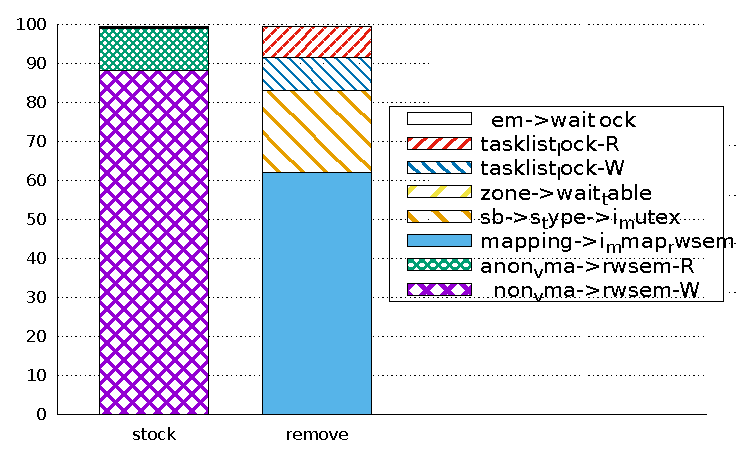
\includegraphics[width=\textwidth]{graph/lockstat}
    \caption{aa}
  \end{subfigure}
  \centering
  \caption{Scalability of AIM7 multiuser. This workload simultaneously create
  many processes.
  Up to 60 core, the stock Linux scale linearly, then they flattens out.}
  \label{fig:aim7_default}
\end{figure}


%운영체제 커널의 paralleism은 시스템 전체의 parallesim에서 가장 중요하다. 
Operating system paralleism is of utmost importance for scalable systems.
%만약에 커널이 scale하지 않으면, 그 위에 동작하는 응용프로그램들도 역시 scale하지 않는다~\cite{Clements15SCR}.
Aplications performance would be limited by the operating system when the
operating system does not scale~\cite{Clements15SCR}[Corey].
% 리눅스는 멀티코어에 최적회된 운영체에 최적화 되어 있기 때문에, 우리는 리눅스에서 AIM7-multiuser를 사용하여
%분석해 보았다.
Linux has heavily optimized for multi-core operating systems, so we examine
AIM7-multiuser benchmark on the Linux.
%AIM7 벤치마크는 최근에도 scalability를 위해 reserach 진영과 리눅스 커널 진영에서도 활발히 이용된다.
% ~\cite{Bueso2015STP}~\cite{Bueso2014MCS}.
The AIM benchmark has, until recently, been widely used in research area
and Linux community~\cite{Bueso2015STP}~\cite{Bueso2014MCS}.
%AIM7-multiuser 워크로드는 동시에 많은 프로세스를 생성하며 수행되며, 디스크 파일 오퍼레이션, 가상 메모리 오퍼레이션, 파이프
%I/O 그리고 수학 연산과 함께 수행한다.
%File system scalability를 최소화 하기 위해 temp filesystem~\cite{Rohland2001Tempfs}을
%사용하였다.
This AIM7-multiuser workload simultaneously creates many processes with
disk-file operations, virtual memory operations, pipe I/O, and arithmetic
operation, and we uses the temp filesystem to minimaize the file system
bottleneck.
%실험 결과 60코어 까지, 리눅스 커널은 확장성이 있으나 그 이후에는 확장성이 떨어져 완만한 그래프를 보여준다. 
The results of scalability shows the stock Linux scales linearly up to 60 core,
then they flattens out(Figure xx(a)).
\fi

%$$$$$$$$$$$$$$$$$$$$$$$$$$$$$$$$$$$$$$$$$$$$$$$$$$$$$$$$$$$$$$$$$$$$$$$$$$$$$$$$
% Paragraph 2: Lockstat로 분석 결과 설명 
%$$$$$$$$$$$$$$$$$$$$$$$$$$$$$$$$$$$$$$$$$$$$$$$$$$$$$$$$$$$$$$$$$$$$$$$$$$$$$$$$

\ifkor
우리는 Scalability에 문제가 있는 120코어에서 리눅스의 Lockstat[]를 이용하여 락 경합을 분석하였다. 
먼저 멀티 프로세스 기반의 벤치마크인 AIM7을 동작시키고 동시에 120코어 대해서 락 경합을 분석하면 
그림 3과 같은 결과를 가진다. 
AIM7 벤치마크의 경우 상당히 많은 부분이 anonvma에서 쓰기 락 경합이 발생한다. 
이는 리눅스 역 매핑(reverse mapping)을 효율적으로 수행하기 위한 자료구인 anonvma가
수많은 fork에 의해 프로세스를 생성하면서 발생하는 락 경합 문제이다. 
이러한 revsers page mapping은 리눅스가 fork(), exit(), and mmap() 시스템콜을 사용할 때 페이지 정보를
update한다.
다음으로 우리는 anonvma의 lock 경합을 줄이기 위해, 임시로 fork에서 anonvma를 호출하는 부분과 read와
관련있는 pageswap이 안되도록 하고, 120코어를 대상으로 다시 Lock 경합을 분석하여 보았다.
이 때 부터 그동안 상대적으로 가려졌던 file reverse mapping에서 많은 락 경합이 발생되었다.
본 연구의 분석 결과 둘 중 하나가 아니라 두 가지 락 모두 fork의 scalabililty 문제를 야기 시킨다.
이러한 anonvma reverse page mapping은 리눅스 커뮤니티에서 잘 알려진 락 경합
문제~\cite{Andi2011adding}~\cite{Tim2013adding}이고, file mapping에 대한 락 경합 문제는
Silas wikizer가 OpLog 논문을 통해 fork의 scalability 문제의 원인으로 제시한 부분이다.
즉 두가지 모두 개선해야지 fork의 scalalbility가 향상 된다. 
\else

%우리는 Scalability에 문제가 있는 120코어에서 리눅스의 Lockstat[]를 이용하여 락 경합을 분석하였다. 
To understand the source of scalability bottleneck on 120core, we profile a lock
contention using the lock\_stat[], a Linux kernel lock profiler that reports how
long each lock is held and the wait time to acquire the lock.
%먼저 멀티 프로세스 기반의 벤치마크인 AIM7을 동작시키고 동시에 120코어 대해서 락 경합을 분석하면 
%그림 3과 같은 결과를 가진다. 
The Figure-xx (b) show the cost of acquiring the lock when the AIM7-multiuser
runs on the 120 core the Linux machine.
%AIM7 벤치마크의 경우 상당히 많은 부분이 anonvma에서 쓰기 락 경합이 발생한다. 
As the result of the lock\_stat, the main problem of lock contention is the
anonymous reverse mapping reader-writer sempaphore(anon\_vma->rwsem).
%이는 리눅스 역 매핑(reverse mapping)을 효율적으로 수행하기 위한 자료구인 anonvma가 수 많은 fork에 의해 프로세스를
% 생성하면서 발생하는 락 경합 문제이다.
, which is generated by simultaneously creating a number of process.
%이러한 revsers page mapping은 리눅스가 fork(), exit(), and mmap() 시스템콜을 사용할 때 페이지 정보를
% update한다.
The reverse page mapping records page information when using fork(), exit() and
mmap() system call to find all page table entries.
%다음으로 우리는 anonvma의 lock 경합을 줄이기 위해, 임시로 fork에서 anonvma를 호출하는 부분과 read와
%관련있는 pageswap이 안되도록 하고, 120코어를 대상으로 다시 Lock 경합을 분석하여 보았다.
%Next we try to use a workaround that remove anon\_vma relative code in the part
%of the fork code with page-swap off avoiding the Linux page reclaiming.
To understand the other bottleneck, we conducted a workaround by removing
anonymous rmap relative code in the part of the fork code with page-swap off
avoding the Linux page reclaiming.
%anon\_vma를 제거하면 리눅스는 file reverse mapping에서 많은 락 경합이 발생되었다.
When the anon\_vma is removed, the Linux is contended on file reverse page
mapping(i\_mmaping-rwsem).
\fi

%$$$$$$$$$$$$$$$$$$$$$$$$$$$$$$$$$$$$$$$$$$$$$$$$$$$$$$$$$$$$$$$$$$$$$$$$$$$$$$$$
% Paragraph 3: 리눅스 reverse page map의 write serialization 문제점
%$$$$$$$$$$$$$$$$$$$$$$$$$$$$$$$$$$$$$$$$$$$$$$$$$$$$$$$$$$$$$$$$$$$$$$$$$$$$$$$$

\ifkor
두가지 revserse page mapping의 근본적인 문제는 hight update operation에 대한 serialization 때문에
발생하는 문제이다.
Update는 execulucive lock을 통해 보호해야하기 때문에, update rate 높은 상황이 발생하면 리눅스
커널은 결국 lock에 의해 serialized되어 scalability가 떨어진다.
\else
%본 연구의 분석 결과 둘 중 하나가 아니라 두 가지 락 모두 fork의 scalabililty 문제를 야기 시킨다.
%이러한 anonvma reverse page mapping은 리눅스 커뮤니티에서 잘 알려진 락 경합
%문제~\cite{Andi2011adding}~\cite{Tim2013adding}이고, file mapping에 대한 락 경합 문제는
%Silas wikizer가 OpLog 논문을 통해 fork의 scalability 문제의 원인으로 제시한 부분이다.
Our research recognized both the anonymous reverse page mapping
reporting from Linux community[] and the file reverse page mapping reporting from S.
Boyd-Wickizer[] are a significant factor in a fork scalability problem.
%즉 두가지 모두 개선해야지 fork의 scalalbility가 향상 된다. 
Thus, in order to perfect scalability of the fork, both the
file reverse mapping and the anonymous reverse mapping should be executed
concurrently without lock.
%두가지 revserse page mapping의 근본적인 문제는 hight update operation에 대한 serialization
%때문에 발생하는 문제이다.
In other word, the fundamental scalability problem of reverse mapping is their
serialized updates operation because operating system kernel are serialized at
the updates operation.

%Update는 execulucive lock을 통해 보호해야하기 때문에, update rate 높은 상황이 발생하면 리눅스
%커널은 결국 lock에 의해 serialized되어 scalability가 떨어진다.


\fi

%$$$$$$$$$$$$$$$$$$$$$$$$$$$$$$$$$$$$$$$$$$$$$$$$$$$$$$$$$$$$$$$$$$$$$$$$$$$$$$$$
% Paragraph 4: update heavy한 상황에 대한 설명과 해결 방법에 대한 설명
%$$$$$$$$$$$$$$$$$$$$$$$$$$$$$$$$$$$$$$$$$$$$$$$$$$$$$$$$$$$$$$$$$$$$$$$$$$$$$$$$

\ifkor
이러한 high update rate이 발생하는 상황의 update serialization 문제에 대한 해결 방법들은 존재한다. 
해결 방법은 concurrent updates를 위한, non-blocking data structure와
log-based 알고리즘을 사용하는 방법이 있다.
Non-blocking algorithms들은 hardware synchronized atomic 연산들을 활용하여 current 하게
update와 read를 수행하게 만든 data structure이다.
하지만 shared memory global value를 multipul CAS로 접근하여 bottlenecks이 생긴다.
due to inter-core communication overheads~\cite{SilasBoydWickizerPth}.
최근에는 Deu to the multipul CAS, inter-core communication overheads를 줄인 log-based
방법들이 연구되고 있다.
우리의 LDU도 이러한 log-based 기반 방법 활용하였으며, log-based 방법에 대한 설명은 다음 장에서 자세히 다룬다.
\else

%이러한 high update rate이 발생하는 상황의 update serialization 문제에 대한 해결 방법들은 존재한다. 
%해결 방법은 concurrent updates를 위한, non-blocking data structure와 log-based 알고리즘을
% 사용하는 방법이 있다.
In order to achieve scalable concurrent update that allows update operations
to proceed without update locks, both the non-blocking
algorithms~\cite{Harris2001Lockfree}~\cite{Fomitchev2004Lockfree}~\cite{Timnat2012}
and log-based algorithms are proposed.
%Non-blocking algorithms들은 hardware synchronized atomic 연산들을 활용하여 current 하게
%update와 read를 수행하게 만든 data structure이다.
In non-blocking algorithms, update operation observes against the current
value in global data structure, and they execute a CAS to compare the against
value.
When the value has been overridden, the updater must be retried.
%하지만 shared memory global value를 multipul CAS로 접근하여 bottlenecks이 생긴다.
%due to inter-core communication overheads~\cite{SilasBoydWickizerPth}.
Consequently, both the repeated CAS operation and the iteration loop caused
by CAS fails will result in bottlenecks due to inter-core communication
overheads~\cite{SilasBoydWickizerPth}.
%최근에는 Deu to the multipul CAS, inter-core communication overheads를 줄인 log-based
%방법들이 연구되고 있다.
To overcome the problem of cache coherence systems, log-based methods are
proposed.
%우리의 LDU도 이러한 log-based 기반 방법 활용하였으며, log-based 방법에 대한 설명은 다음 장에서 자세히 다룬다.
Our research also uses a log-based deferred design that alows concurrent
updates to scale, so that multiprocessed applications can scale to large numbers of cores.
%The next section explains our log-based algorithm.
\fi

\subsection{Log-based Concurrent updates}

%$$$$$$$$$$$$$$$$$$$$$$$$$$$$$$$$$$$$$$$$$$$$$$$$$$$$$$$$$$$$$$$$$$$$$$$$$$$$$$$$
%Paragraph 1: Log 기반의 알고리즘 대략적인 설명 
%$$$$$$$$$$$$$$$$$$$$$$$$$$$$$$$$$$$$$$$$$$$$$$$$$$$$$$$$$$$$$$$$$$$$$$$$$$$$$$$$

\ifkor
Update heavy한 자료구조 때문에 발생하는 scalability 문제에 대한 해결책 중 하나는 Log-based 알고리즘을 사용하는
것이다.
Log-based 알고리즘은 lock을 피하기 위해 update가 발생하면, data structure의 update
operation(insert or remove)을 argument와 함께 저장하고, 주기적 또는 read operation을 수행하기 전에
applies the updates in all the logs to the data structure, so reader can read up to date data structure.
이러한 Log-based 방법은 마치 CoW(Copy on Write)와 유사하다.
즉, read 전에 저장된 log가 수행됨으로 read가 간혈적으로 수행되는 data structure에 적합한 방법이다.
\else
%Log-based 알고리즘은 lock을 피하기 위해 update가 발생하면, data structure의 update
%operation(insert or remove)을 argument와 함께 저장하고, 주기적 또는 read operation을 수행하기 전에
%applies the updates in all the logs to the data structure, so reader can read
% up to date data structure.
Log-based algorithm is that when update operations occur, it logs the update
operation and applies the all operation logs to the data structure
before read operation, so reader can read up to date data structure;it similar
to CoW(Copy On Write)~\cite{PaulDetailLWN}.

%Update heavy한 자료구조 때문에 발생하는 scalability 문제에 대한 해결책 중 하나는 Log-based 알고리즘을 사용하는
%것이다.
The log-based algorithms~\cite{Hendler2010FC}~\cite{SilasBoydWickizerPth} are
the suitable solution for update-heavy data structure because it alows update
operations to proceed with a coarse grained update lock or without update locks.
The benefit of avoiding fine grained update lock can eliminate the overhead of
acquiring a lock requires fetching the lock's cache line from the core that
last updated the lock status.
Thus, it reduces the cache communication traffic;a contended cache line on
many-core processors can take hundreds of cycles to fetch from a remote
core[], and these techniques can be easily applied to other data structures.
In addition to avoid fine grained lock and easily apply the
other data structure, a log-based method can removes the existing
operation log rather than actually executing the operation log.
%이러한 Log-based 방법은 마치 CoW(Copy on Write)와 유사하다.
%즉, read 전에 저장된 log가 수행됨으로 read가 간혈적으로 수행되는 data structure에 적합한 방법이다.
\fi

%$$$$$$$$$$$$$$$$$$$$$$$$$$$$$$$$$$$$$$$$$$$$$$$$$$$$$$$$$$$$$$$$$$$$$$$$$$$$$$$$
%Paragraph 2: Log 기반의 알고리즘의 장점
%$$$$$$$$$$$$$$$$$$$$$$$$$$$$$$$$$$$$$$$$$$$$$$$$$$$$$$$$$$$$$$$$$$$$$$$$$$$$$$$$
%
\ifkor
Update heavy한 구조를 위한 Log-based 방법은 총 4가지의 장점을 가진다. 
첫째로, update가 수행하는 시점 즉 로그를 저장하는 순간에는 lock이 필요가 없다. 
따라서 update를 concurrent하게 수행할 수 있을 뿐아니라, lock 자체가 가지고 있는 overall
coherence traffic is significantly reduced.
둘째로, 저장된 sequantial update operation log를 corse-grain lock과 함께 하나의 코어에서 수행하기
때문에, cache 효율성이 높아진다.
셋째로, 큰 수정 없이 기존 여러 데이터(tree, queue) structure에 쉽게 적용할 수 있는 장점이 있다.
마지막으로 저장된 log를 실제 수행하지 않고, 여러가지 optimization 방법을 사용하여 적은 operation으로 Log를 줄일 수
있다. 
LDU도 log-based approach를 따른다. 그러므로 앞에서 설명한 log-based 방법의 장점을 모두 가짐과 동시에
업데이트 순간 삭제 가능한 log를 지움으로 성능을 향상시킨다.
\else
\fi


%$$$$$$$$$$$$$$$$$$$$$$$$$$$$$$$$$$$$$$$$$$$$$$$$$$$$$$$$$$$$$$$$$$$$$$$$$$$$$$$$
%$$$$$$$$$$$$$$$$$$$$$$$$$$$$$$$$$$$$$$$$$$$$$$$$$$$$$$$$$$$$$$$$$$$$$$$$$$$$$$$$
%Reference Sentence 1





%$$$$$$$$$$$$$$$$$$$$$$$$$$$$$$$$$$$$$$$$$$$$$$$$$$$$$$$$$$$$$$$$$$$$$$$$$$$$$$$$
%Reference Sentence 2:LDU paper
%$$$$$$$$$$$$$$$$$$$$$$$$$$$$$$$$$$$$$$$$$$$$$$$$$$$$$$$$$$$$$$$$$$$$$$$$$$$$$$$$




